\documentclass{article}

\usepackage{xstring}
\usepackage{fancyhdr}
\usepackage{extramarks}
\usepackage{amsmath}
\usepackage{amsthm}
\usepackage{amsfonts}
\usepackage{tikz}
\usepackage[plain]{algorithm}
\usepackage{algpseudocode}
\usepackage{parskip}
\usepackage{enumerate}
\usepackage{setspace}
\usetikzlibrary{arrows,shapes,positioning,shadows,trees}

%
% Basic Document Settings
%

\topmargin=-0.45in
\evensidemargin=0in
\oddsidemargin=0in
\textwidth=6.5in
\textheight=9.0in
\headsep=0.25in

\linespread{1.1}

\pagestyle{fancy}
\lhead{\hmwkAuthorName}
\chead{\hmwkClass\ (\hmwkClassInstructor): \hmwkTitle}
\rhead{\firstxmark}
\lfoot{\lastxmark}
\cfoot{\thepage}

\renewcommand\headrulewidth{0.4pt}
\renewcommand\footrulewidth{0.4pt}

\setlength\parindent{0pt}

\tikzset{
    raw sort entry/.style={rectangle, thick, draw, node distance=1.5em, align=center},
    sort entry black/.style={raw sort entry, black, fill=white, align=center},
    p1/.style={raw sort entry, black, fill=gray!25},
    s1/.style={raw sort entry, red, fill=yellow!30},
    s2/.style={raw sort entry, blue, fill=green!20},
    s3/.style={raw sort entry, violet, fill=orange!25},
    basic/.style  = {draw, font=\sffamily, rectangle},
    root/.style   = {basic, rounded corners=2pt, thin, align=center},
    level 2/.style = {basic, rounded corners=6pt, thin,align=center},
    level 3/.style = {basic, thin, align=left}
}

\newcommand*{\List}[2][sort entry black]{%
  \par\noindent%
  \edef\listtoprocess{#2}%
  \def\ListToProcess{}%
  \begin{center}
  \begin{tikzpicture}[inner sep=2pt, outer sep=0]
    \foreach \content in \listtoprocess{
      \IfSubStr{\content}{/}{% true
        \xdef\ListToProcess{\ListToProcess,\content}
      }{%                      false
        \xdef\ListToProcess{\ListToProcess,#1/\content}
      }
    }
    \StrGobbleLeft{\ListToProcess}{1}[\ListToProcess]% removes the first comma (\listToProcess is empty at the start)
    \foreach [count=\i] \Style/\Value in \ListToProcess {
      \ifnum\i=1\relax
        \node [raw sort entry, \Style] (sortnode\i) {\Value};
      \else
        \node [raw sort entry, right of=sortnode\number\numexpr\i-1\relax, \Style] (sortnode\i) {\Value};
      \fi
    }
  \end{tikzpicture}%
  \end{center}
}

%
% Create Problem Sections
%

\newcommand{\enterProblemHeader}[1]{
    \nobreak\extramarks{}{Problem \arabic{#1} continued on next page\ldots}\nobreak{}
    \nobreak\extramarks{Problem \arabic{#1} (continued)}{Problem \arabic{#1} continued on next page\ldots}\nobreak{}
}

\newcommand{\exitProblemHeader}[1]{
    \nobreak\extramarks{Problem \arabic{#1} (continued)}{Problem \arabic{#1} continued on next page\ldots}\nobreak{}
    \stepcounter{#1}
    \nobreak\extramarks{Problem \arabic{#1}}{}\nobreak{}
}

\setcounter{secnumdepth}{0}
\newcounter{partCounter}
\newcounter{homeworkProblemCounter}
\setcounter{homeworkProblemCounter}{1}
\nobreak\extramarks{Problem \arabic{homeworkProblemCounter}}{}\nobreak{}

%
% Homework Problem Environment
%
% This environment takes an optional argument. When given, it will adjust the
% problem counter. This is useful for when the problems given for your
% assignment aren't sequential. See the last 3 problems of this template for an
% example.
%
\newenvironment{homeworkProblem}[1][-1]{
    \ifnum#1>0
        \setcounter{homeworkProblemCounter}{#1}
    \fi
    \section{Problem \arabic{homeworkProblemCounter}}
    \setcounter{partCounter}{1}
    \enterProblemHeader{homeworkProblemCounter}
}{
    \exitProblemHeader{homeworkProblemCounter}
}

%
% Homework Details
%   - Title
%   - Due date
%   - Class
%   - Section/Time
%   - Instructor
%   - Author
%

\newcommand{\hmwkTitle}{Sorting Algorithms}
\newcommand{\hmwkDueDate}{February 26, 2015}
\newcommand{\hmwkClass}{CS350 - Algorithms}
\newcommand{\hmwkClassInstructor}{for Professor Andrew Black}
\newcommand{\hmwkAuthorName}{Kristina Frye}

%
% Title Page
%

\title{
    \vspace{2in}
    \textmd{\textbf{\hmwkClass:\ \hmwkTitle}}\\
    \normalsize\vspace{0.1in}\small{Due\ on\ \hmwkDueDate}\\
    \vspace{0.1in}\large{\textit{\hmwkClassInstructor}}
    \vspace{3in}
}

\author{\textbf{\hmwkAuthorName}}
\date{}

\renewcommand{\part}[1]{\textbf{\large Part \Alph{partCounter}}\stepcounter{partCounter}\\}

%
% Various Helper Commands
%

% Useful for algorithms
\newcommand{\alg}[1]{\textsc{\bfseries \footnotesize #1}}

% For derivatives
\newcommand{\deriv}[1]{\frac{\mathrm{d}}{\mathrm{d}x} (#1)}

% For partial derivatives
\newcommand{\pderiv}[2]{\frac{\partial}{\partial #1} (#2)}

% Integral dx
\newcommand{\dx}{\mathrm{d}x}

% Alias for the Solution section header
\newcommand{\solution}{\textbf{\large Solution}}

% Probability commands: Expectation, Variance, Covariance, Bias
\newcommand{\E}{\mathrm{E}}
\newcommand{\Var}{\mathrm{Var}}
\newcommand{\Cov}{\mathrm{Cov}}
\newcommand{\Bias}{\mathrm{Bias}}

\begin{document}

\pagebreak

\begin{figure}[quicksort]\begin{doublespace}
\List{s2/3, 5, 7, 1, p1/2, 12, 0, 2, 8, s3/1} 
\List{1, s2/5, 7, 1, p1/2, 12, 0, s3/2, 8, 3}
\List{1, 2, s2/7, 1, p1/2, 12, s3/0, 5, 8, 3}
\List{s2/1, p1/2, 0, s3/1, , 2, , s2/12, 7, p1/5, 8, s3/3}
\List{1, s2/2, 0, s3/1, , 2, , 3, s2/7, s3/5, 8, 12}
\List{1, 1, 0, p1/2, , 2, , 3, p1/5, 7, 8, 12}
\List{s2/1, p1/1, s3/0,, 2, , 2, , 3,, 5,, s2/7, p1/8, s3/12}
\List{0, p1/1, 1,, 2, , 2, , 3,, 5,, 7, p1/8, 12}
\List{0, 1, 1,2, 2, 3, 5, 7, 8, 12}
\caption{Quicksort: the blue and red boxes represent the values to be swapped. The 
grey box represents the pivot.}\end{doublespace}
\end{figure}

\section{Mergesort}
Mergesort is a divide-and-conquer algorithm in which the unsorted array is recursively divided
in half until each subarray has only one element. Then the pieces are merged back together in 
order, eventually recombining back into one sorted array. See Figure~\ref{pseudo-mergesort} for the pseudocode representation of Mergesort.

In the first phase of Mergesort, the elements of the array are copied $\log_2(n)$ times until each 
element is in its own subarray. Although no comparisons are made in this phase of the algorithm,
this does require $n\log_2 n$ copy operations (each element is copied $\log_2n$ times) 
and doubles the required space allocation for the array.

In the second phase of Mergesort, the elements of each subarray are combined. In the worst case, 
each of the two subarrays being combined into one array is reduced by one after each comparison
until both arrays are empty, for a total of $n-1$ comparisons. Adding these comparisons to the
number of comparisons that were done to create each of the subarrays gives the following
recurrence:
\[
	C(n) = 2 \cdot C\left(\frac{n}{2}\right) + n-1, C(1) = 0
\]
This recurrence is conveniently in the form of the Master Theorem in which
\[
	T(n) = a \cdot T\left(\frac{n}{b}\right) +f(n)
\]
and $f(n) \in \Theta(n^d)$. For Mergesort, $a = 2, b = 2, d = 1$ and $a = 2 = 2^1 = b^d$. 
Therefore, according to the Master Theorem, $C(n) \in \Theta(n^d \log n)$. However, in many
cases, there will need to be less than $n-1$ comparisons in each merge. For instance, if
all the elements of the left subarray are less than all the elements of the right array, then after
$\frac{n}{2}$ comparisons after which each element of the left array is placed into the sorted array,
the elements of the right array can simply be copied to the sorted array without any other
comparisons. See line~\ref{line:mergesort1} through line~\ref{line:mergesort2} in Figure~\ref{pseudo-mergesort}.

Figure~\ref{example-mergesort} shows an example of an array of numbers being sorted with Mergesort.

Mergesort has many advantages. First of all, our of all the "good" sorting algorithms, it is probably
the easiest to understand and thus implement. Also, its worst case is better than the worst
case of Quicksort, which is generally considered a faster algorithm. But its main advantage is that,
unlike many other sorting algorithms, it is a \textit{stable} sort. That is, two elements that are equal 
to each other will remain in the same relative order after the algorithm has been completed. 

Mergesort has two main disadvantages. First, it requires a large number of copy operations in both
phases of the algorithm. Second, it requires $O(n)$ of extra space and cannot be performed 
in place.

\begin{figure}
\begin{algorithmic}[1]
	\Procedure{Mergesort}{$A[0..n-1]$}
		\State $left \gets A[0..n/2]$
		\State $right \gets A[n/2 + 1..n-1]$
		\State $left \gets Mergesort(left)$
		\State $right \gets Mergesort(right)$
		\State $A \gets merge(left, right, A)$
	\EndProcedure
	
	\Procedure{Merge}{$left, right$}
		\State $i \gets 0$
		\State $j \gets 0$
		\State $k \gets 0$
		\While{$i < left.length$ AND $j < right.length$}
			\If {$left[i] < right[j]}$
				\State $A[k] \gets left[i]$
				\State $i \gets i + 1$
			\Else
				\State $A[k] \gets right[j]$
				\State $j \gets j + 1$
			\EndIf
			\State $k \gets k + 1$
		\EndWhile
		\If {$i = left.length$} \label{line:mergesort1}
			\State copy $right[j..right.length - 1]$ to $A[k..left.length + right.length - 1]$
		\Else
			\State copy $left[i..left.length - 1]$ to $A[k..left.length + right.length - 1]$
		\EndIf \label{line:mergesort2}
		\State return $A$
	\EndProcedure
\end{algorithmic}
\caption{Pseudocode for Mergesort}
\label{pseudo-mergesort}
\end{figure}
	
\begin{figure}[mergesort] \begin{center}
	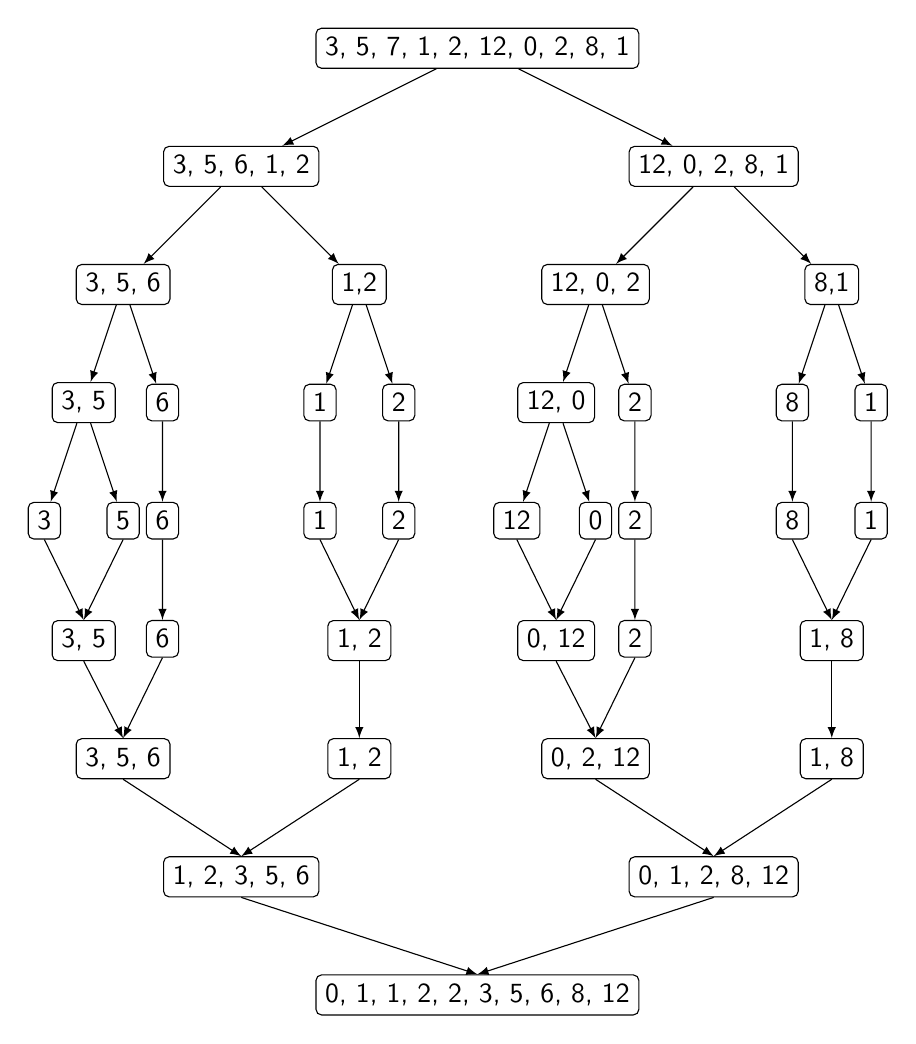
\begin{tikzpicture}[
	level 1/.style={sibling distance=60mm},
	level 2/.style={sibling distance=30mm},
	level 3/.style={sibling distance=10mm},
	edge from parent/.style={->,draw},>=latex]
		\begin{scope}[every node/.style={root}]
			\node(node35712120281){3, 5, 7, 1, 2, 12, 0, 2, 8, 1}
			child {node(node35612){3, 5, 6, 1, 2}
				child {node(node356-1){3, 5, 6}
					child{node(node35-1){3, 5}
						child{node(node3){3}}
						child{node(node5){5}}}
					child{node{6}
						child{node{6}
						child{node(node6){6}}}}}
				child {node(node12-1){1,2}
					child{ node{1}
						child{ node(node1){1}}}
					child{ node{2}
						child{ node(node2){2}}}}}
			child {node(node120281){12, 0, 2, 8, 1}
				child {node(node1202){12, 0, 2}
					child{ node(node120){12, 0}
						child{ node(node12-4){12}}
						child{ node(node0){0}}}
					child{ node{2}
						child{ node{2}
							child{ node(node2-2){2}}}}}
				child {node(node81){8,1}
					child{ node{8}
						child{ node(node8){8}}}
					child { node{1}
						child{ node(node1-2){1}}}}};
		\node[below = 2.5 of node35-1](node35-2){3, 5};
		\draw[->] (node3.south) --  (node35-2.north);
		\draw[->] (node5.south) --  (node35-2.north);
		
		\node[below = 4 of node12-1](node12-2){1, 2}
			child{ node(node12-3){1, 2}};
		
		\node[below = 2.5 of node120](node012){0, 12};
		\draw[->] (node12-4.south) --  (node012.north);
		\draw[->] (node0.south) --  (node012.north);
		\draw[->] (node1.south) --  (node12-2.north);
		\draw[->] (node2.south) --  (node12-2.north);
		
		\node[below = 4 of node81](node18){1, 8}
			child{ node(node18-2){1, 8}};
		\draw[->] (node8.south) --  (node18.north);
		\draw[->] (node1-2.south) --  (node18.north);
		
		\node[below = 5.5 of node1202](node0212){0, 2, 12};
		\draw[->] (node012.south) --  (node0212.north);
		\draw[->] (node2-2.south) --  (node0212.north);
		
		\node[below = 5.5 of node356-1](node356-2){3, 5, 6};
		\draw[->] (node35-2.south) --  (node356-2.north);
		\draw[->] (node6.south) --  (node356-2.north);
		\node[below = 8.5 of node35612](node12356){1, 2, 3, 5, 6};
		\draw[->] (node356-2.south) -- (node12356.north);
		\draw[->] (node12-3.south) -- (node12356.north);
		
		\node[below = 8.5 of node120281](node012812){0, 1, 2, 8, 12};
		\draw[->] (node0212.south) -- (node012812.north);
		\draw[->] (node18-2.south) -- (node012812.north);
		
		\node[below = 11.5 of node35712120281](end){0, 1, 1, 2, 2, 3, 5, 6, 8, 12};
		\draw[->] (node12356.south) -- (end.north);
		\draw[->] (node012812.south) -- (end.north);
		\end{scope}
	\end{tikzpicture} \caption{An example of Mergesort} \label{example-mergesort}
\end{center} \end{figure}
\pagebreak

\begin{figure}
\begin{algorithmic}
	\Procedure{3WayQS}{$A[l..r]$}
		\If{ $l > r$}
			\State \textbf{return}
		\EndIf

		\State $left \gets l$
		\State $right \gets r$
		\State $i \gets l + 1$
		\State $pivotIdx \gets l$
		\State $pivotVal \gets A[pivotIdx]$

		\While{$i <= right$}
  			\If{$A[i] < pivotVal$}
				\State $swap(A[i], A[left]$
    				\State $left \gets left + 1$
    				\State $i \gets i + 1$
  			\Else
				\If{$pivotVal < A[i]$}
					\State $swap(A[i], A[right])$
    					\State $right \gets right - 1$
  				\Else
    					\State $i \gets i + 1$
				\EndIf
			\EndIf
		\EndWhile
		\State $3WayQS(l, left - 1)$
		\State $3WayQS(right + 1, r)$
	\EndProcedure
\end{algorithmic}
\end{figure}

\begin{figure}[3wayquicksort]\begin{doublespace}
\List{s2/3, 5, 7, 1, 2, 12, 0, 2, 8, s3/1} 
\List{1, s2/5, 7, 1, 2, 12, 0, 2, s3/8, 3}
\List{1, s2/8, 7, 1, 2, 12, 0, s3/2, 5, 3}
\List{1, 2, s2/7, 1, 2, 12, s3/0, 8, 5, 3}
\List{1, s2/2, s3/0, 1, 2, 12, 7, 8, 5, 3}
\List{s2/1, s3/0, 2, 1, 2, 12, 7, 8, 5, 3}
\List{0, 1, 2, 1, 2, s2/12, 7, 8, 5, s3/3}
\List{0, , 1, , s2/2, s3/1, 2, ,3, ,7, 8, 5, 12}
\List{0, , 1, , 1, 2, 2, ,3, ,7, s2/8, s3/5, 12}
\List{0, , 1, , 1, 2, 2, ,3, ,s2/7, s3/5, , 8, 12}
\List{0, 1, 1, 2, 2, 3, 5, 7, 8, 12}
\caption{3 Way Quicksort: the blue and red boxes represent the values to be swapped. The 
grey box represents the pivot.}\end{doublespace}
\end{figure}

\pagebreak
\begin{figure}
\begin{algorithmic}
	\Procedure{DualPivotQS}{$A[l..r]$}
		\If{$l > r$}
  			\State \textbf{return}
		\EndIf
		\State $left \gets l$
		\State $right \gets r$
		\State $i \gets l + 1$
		\If{$A[l] > A[r]$}
  			\State $temp \gets A[l]$
  			\State $A[l] \gets A[r]$
  			\State $A[r] \gets temp$
		\EndIf
		\While{$i <= right$}
  			\If{$A[i] < A[l]$}
    				\State $swap(A[i], A[left$
    				\State $left \gets left + 1$
				\State $i \gets i + 1$
  			\Else 
				\If{$A[r] < A[i]$}
    					\State $swap(A[i], A[right]$
    					\State $right \gets right - 1$
  				\Else
    					\State $i \gets i + 1$
				\EndIf
			\EndIf
		\EndWhile
		\State $left \gets left - 1$
		\State $swap(A[left], A[l])$
		\State $right \gets right + 1$
		\State $swap(A[right], A[r])$
		\State $DualPivotQS(l, left - 1)$
		\If{$A[left] < A[right]$}
  			\State $DualPivotQS(left + 1, right - 1)$
		\EndIf
		\State $DualPivotSort(right + 1, r)$
	\EndProcedure
\end{algorithmic}
\end{figure}
\pagebreak

\begin{figure}[quicksort]\begin{doublespace}
	\List{p1/3, s2/5, 7, 1, 2, 12, 0, 2, 8, s3/1} 
	\List{s2/3, s3/1, 7, 1, 2, 12, 0, 2, 8, 5}
	\List{1, p1/3, s2/7, 1, 2, 12, 0, 2, s3/8, 5}
	\List{1, p1/3, s2/8, 1, 2, 12, 0, 2, s3/7, 5}
	\List{1, s2/3, s3/2, 1, 2, 12, 0, 8, 7, 5}
	\List{1, 2, s2/3, s3/1, 2, 12, 0, 8, 7, 5}
	\List{1, 2, 1, s2/3, s3/2, 12, 0, 8, 7, 5}
	\List{1, 2, 1, 2, p1/3, s2/12, s3/0, 8, 7, 5}
	\List{1, 2, 1, 2, s2/3, s3/0, 12, 8, 7, 5}
	\List{1, 2, 1, 2, 0, p1/3, 12, 8, 7, 5}
	\List{p1/1, s2/2, 1, 2, s3/0, , 3, , s2/12, s3/8, 7, 5}
	\List{s2/1, s3/0, 1, 2, 2, , 3, , 8, s2/12, s3/7, 5}
	\List{0, p1/1, 1, 2, 2, , 3, , 8, 7, s2/12, s3/5}
	\List{0, p1/1, 1, 2, 2, , 3, , 8, 7, 5, p1/12}
	\List{0, p1/1, 1, 2, 2, , 3, , s2/8, s3/7, 5, 12}
	\List{0, p1/1, 1, 2, 2, , 3, , 7, s2/8, s3/5, 12}
	\List{0, p1/1, 1, 2, 2, , 3, , 7, 5, p1/8, 12}
	\List{0, p1/1, 1, 2, 2, , 3, , s2/7, s3/5, 8, 12}
	\List{0, p1/1, 1, 2, 2, , 3, , 5, 7, 8, 12}
\caption{3 Way Sort}\end{doublespace}
\end{figure}

\pagebreak
\begin{figure}
\begin{algorithmic}
	\Procedure{Heapsort}{$A[0..n-1], lo, high$}
		\State $length \gets high - lo$
		\For {$i := length/2 \text{ to } 1 \textbf{ step } {-1}$}
			\State $heap(A, i, length, lo)$
		\EndFor
		\For {$i := length - 1 \text{ to } 0 \textbf{ step }{-1}$}
			\State $swap(A, lo, lo + i - 1)$
			\State $heap(A, 1, i-1, lo)$
		\EndFor
	\EndProcedure
	
	\Procedure{heap}{$A[0..n-1], root, bottom, lo)$}
		\State $d \gets A[lo + root - 1]$
		\While{$root * 2 \le bottom$}
			\State $child \gets 2 * root$
			\If{$child < bottom$ AND $A[lo + child - 1] \le A[lo + child]$}
				\State $child \gets child + 1$
			\EndIf
			\If{$d \ge A[lo + child - 1$}
				\State break
			\EndIf
			\State $A[lo + root - 1] = A[lo + child - 1]$
			\State $root = child$
		\EndWhile
		\State $A[lo + root - 1] \gets d$
	\EndProcedure
\end{algorithmic}
\end{figure}

\begin{figure}[heapsort]
	\List{3, 5, 7, 1, 2, 12, 0, 2, 8, 1}
	\vspace{5mm}
	\begin{center}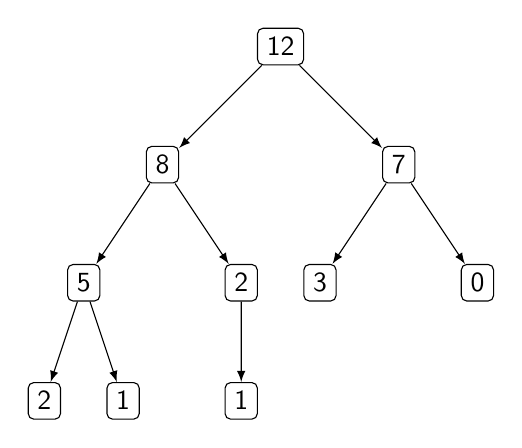
\begin{tikzpicture}[
	level 1/.style={sibling distance=30mm},
	level 2/.style={sibling distance=20mm},
	level 3/.style={sibling distance=10mm},
	edge from parent/.style={->,draw},>=latex]
		\begin{scope}[every node/.style={root}]
			\node{12}
				child{node{8}
					child{ node{5}
						child{ node{2}}
						child{ node{1}}}
					child{ node{2}
						child{ node{1}}}}
				child{ node{7}
					child{ node{3}}
					child{ node{0}}};	
		\end{scope}
	\end{tikzpicture}\end{center} 
\caption{Heapsort}\end{figure}

\begin{figure}[heapsort2]
	\List{1, 8, 7, 5, 2, 3, 0, 2, 1, 12}
	\vspace{5mm}
	\begin{center}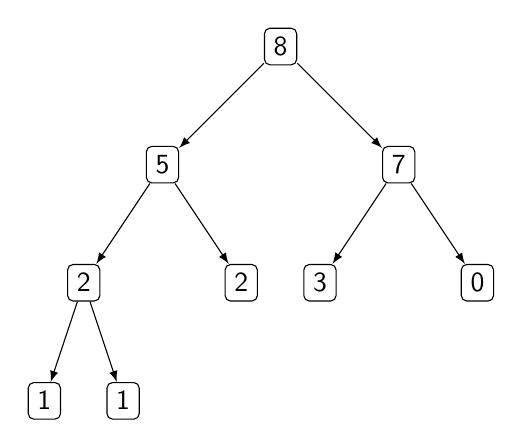
\begin{tikzpicture}[
	level 1/.style={sibling distance=30mm},
	level 2/.style={sibling distance=20mm},
	level 3/.style={sibling distance=10mm},
	edge from parent/.style={->,draw},>=latex]
		\begin{scope}[every node/.style={root}]
			\node{8}
				child{node{5}
					child{node{2}
						child{node{1}}
						child{node{1}}}
					child{node{2}}}
				child{node{7}
					child{node{3}}
					child{node{0}}};
		\end{scope}
	\end{tikzpicture}\end{center} 
\end{figure}

\begin{figure}[heapsort2]
	\List{1, 5, 7, 2, 2, 3, 0, 1, 8, 12}
	\vspace{5mm}
	\begin{center}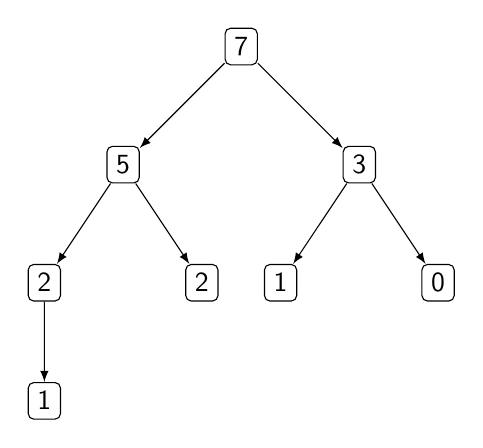
\begin{tikzpicture}[
	level 1/.style={sibling distance=30mm},
	level 2/.style={sibling distance=20mm},
	level 3/.style={sibling distance=10mm},
	edge from parent/.style={->,draw},>=latex]
		\begin{scope}[every node/.style={root}]
			\node{7}
				child{node{5}
					child{node{2}
						child{node{1}}}
					child{node{2}}}
				child{node{3}
					child{node{1}}
					child{node{0}}};
		\end{scope}
	\end{tikzpicture}\end{center} 
\end{figure}
	
\begin{figure}[heapsort2]
	\List{1, 5, 3, 2, 2, 1, 0, 7, 8, 12}
	\vspace{5mm}
	\begin{center}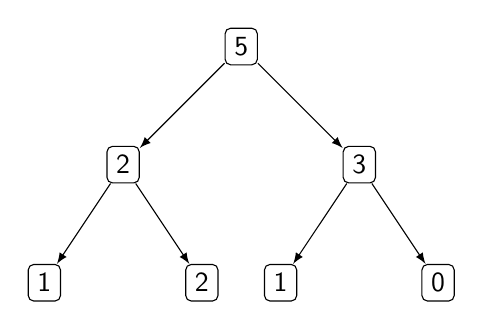
\begin{tikzpicture}[
	level 1/.style={sibling distance=30mm},
	level 2/.style={sibling distance=20mm},
	level 3/.style={sibling distance=10mm},
	edge from parent/.style={->,draw},>=latex]
		\begin{scope}[every node/.style={root}]
			\node{5}
				child{node{2}
					child{node{1}}
					child{node{2}}}
				child{node{3}
					child{node{1}}
					child{node{0}}};
		\end{scope}
	\end{tikzpicture}\end{center} 
\end{figure}

\begin{figure}[heapsort2]
	\List{0, 2, 3, 1, 2, 1, 5, 7, 8, 12}
	\vspace{5mm}
	\begin{center}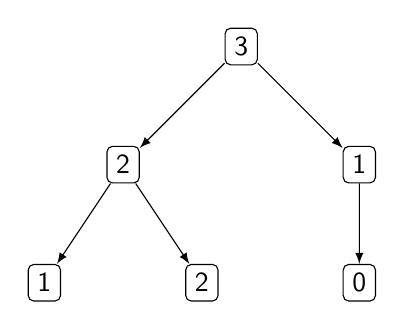
\begin{tikzpicture}[
	level 1/.style={sibling distance=30mm},
	level 2/.style={sibling distance=20mm},
	level 3/.style={sibling distance=10mm},
	edge from parent/.style={->,draw},>=latex]
		\begin{scope}[every node/.style={root}]
			\node{3}
				child{node{2}
					child{node{1}}
					child{node{2}}}
				child{node{1}
					child{node{0}}};
		\end{scope}
	\end{tikzpicture}\end{center} 
\end{figure}

\begin{figure}[heapsort2]
	\List{0, 2, 1, 1, 2, 3, 5, 7, 8, 12}
	\vspace{5mm}
	\begin{center}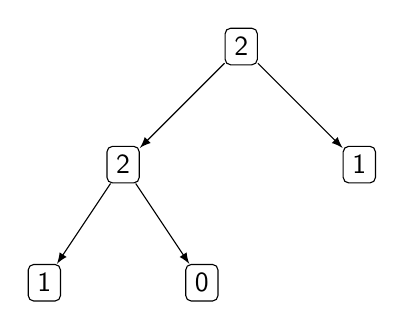
\begin{tikzpicture}[
	level 1/.style={sibling distance=30mm},
	level 2/.style={sibling distance=20mm},
	level 3/.style={sibling distance=10mm},
	edge from parent/.style={->,draw},>=latex]
		\begin{scope}[every node/.style={root}]
			\node{2}
				child{node{2}
					child{node{1}}
					child{node{0}}}
				child{node{1}};
		\end{scope}
	\end{tikzpicture}\end{center} 
\end{figure}	
\begin{figure}[heapsort2]
	\List{0, 2, 1, 1, 2, 3, 5, 7, 8, 12}
	\vspace{5mm}
	\begin{center}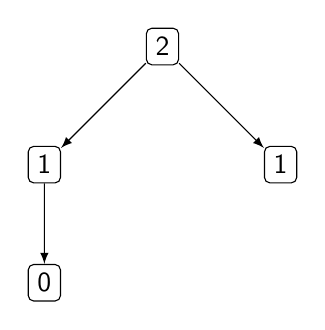
\begin{tikzpicture}[
	level 1/.style={sibling distance=30mm},
	level 2/.style={sibling distance=20mm},
	level 3/.style={sibling distance=10mm},
	edge from parent/.style={->,draw},>=latex]
		\begin{scope}[every node/.style={root}]
			\node{2}
				child{node{1}
					child{node{0}}}
				child{node{1}};
		\end{scope}
	\end{tikzpicture}\end{center} 
\end{figure}

\begin{figure}[heapsort2]
	\List{0, 1, 1, 2, 2, 3, 5, 7, 8, 12}
	\vspace{5mm}
	\begin{center}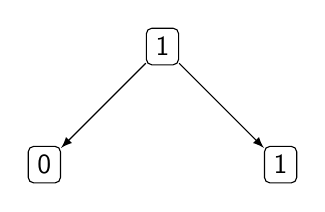
\begin{tikzpicture}[
	level 1/.style={sibling distance=30mm},
	level 2/.style={sibling distance=20mm},
	level 3/.style={sibling distance=10mm},
	edge from parent/.style={->,draw},>=latex]
		\begin{scope}[every node/.style={root}]
			\node{1}
				child{node{0}}
				child{node{1}};
		\end{scope}
	\end{tikzpicture}\end{center} 
\end{figure}

\begin{figure}[heapsort2]
	\List{1, 0, 1, 2, 2, 3, 5, 7, 8, 12}
	\vspace{5mm}
	\begin{center}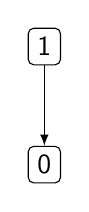
\begin{tikzpicture}[
	level 1/.style={sibling distance=30mm},
	level 2/.style={sibling distance=20mm},
	level 3/.style={sibling distance=10mm},
	edge from parent/.style={->,draw},>=latex]
		\begin{scope}[every node/.style={root}]
			\node{1}
				child{node{0}};
		\end{scope}
	\end{tikzpicture}\end{center} 
	\vspace{5mm}
	\List{0, 1, 1, 2, 2, 3, 5, 7, 8, 12}
\end{figure}

\end{document}
